\documentclass[xcolor=dvipsnames
              %,handout
              ]{beamer} 

\usetheme{Madrid} 
%\setbeamertemplate{blocks}[shadow=false] 
\setbeamertemplate{navigation symbols}{} 
\setbeamertemplate{items}[square]
\setbeamertemplate{sections/subsections in toc}[square]

\definecolor{myblueend}{rgb}{0.058,0.132,0.42}
\definecolor{mybluemiddle}{rgb}{0.31,0.45,0.64}
\definecolor{mybluestart}{rgb}{0.17,0.28,0.48}
\definecolor{mygreen}{rgb}{0,0.7,0}
\definecolor{mylightgreen}{rgb}{0.7,1,0.7}
\definecolor{mylightblue}{rgb}{0.7,0.7,1}
\definecolor{mylightblack}{rgb}{0.7,0.7,0.7}
\definecolor{mylightred}{rgb}{1,0.7,0.7}
\definecolor{oproverblue}{RGB}{12,83,144}
\definecolor{oproveryellow}{RGB}{255,156,55}
\definecolor{mydarkgreen}{rgb}{0.17,0.48,0.28}
\definecolor{mydarkred}{rgb}{0.48,0.28,0.17}
\definecolor{grey}{rgb}{0.7,0.7,0.7}
\definecolor{darkgrey}{rgb}{0.5,0.5,0.5}

%\setbeamercolor{palette primary}{fg=white,bg=mybluestart}
%\setbeamercolor{palette secondary}{fg=white,bg=mybluestart}
%\setbeamercolor{palette tertiary}{fg=white,bg=mybluestart}
%\setbeamercolor{palette quaternary}{fg=white,bg=mybluestart}
\setbeamercolor{palette primary}{fg=white,bg=oproverblue}
\setbeamercolor{palette secondary}{fg=white,bg=oproverblue}
\setbeamercolor{palette tertiary}{fg=white,bg=oproverblue}
\setbeamercolor{palette quaternary}{fg=white,bg=oproverblue}
\setbeamercolor{titlelike}{parent=palette quaternary}

\setbeamercolor{item}{fg=oproverblue}
\setbeamercolor{block title}{fg=white,bg=oproverblue}
\setbeamercolor{block title example}{fg=white,bg=oproveryellow}
%\setbeamercolor{block title alert}{fg=white,bg=mydarkred}

\usefonttheme{serif}

%%
%% TOOLS
%% 
\newcommand{\opensmt}{{\sc OpenSMT}\xspace}
\newcommand{\yices}{{\sc Yices}\xspace}
\newcommand{\mathsat}{{\sc MathSAT}\xspace}
\newcommand{\cvcfour}{{\sc CVC4}\xspace}
\newcommand{\zthree}{{\sc Z3}\xspace}
\newcommand{\boolector}{{\sc Boolector}\xspace}
\newcommand{\verit}{{\sc veriT}\xspace}
\newcommand{\stp}{{\sc STP}\xspace}
\newcommand{\minisat}{{\sc MiniSAT}\xspace}
%%
%% BOOLEAN OPERATORS
%%
\newcommand{\swedge}{\,\wedge\,}
\newcommand{\svee}{\,\vee\,}
\newcommand{\impl}{\,\rightarrow\,}
%%
%% SMTLIB LOGICS
%% 
\newcommand{\Idl}{\ensuremath{\mathcal{IDL}}\xspace}
\newcommand{\Rdl}{\ensuremath{\mathcal{RDL}}\xspace}
\newcommand{\Uf}{\ensuremath{\mathcal{UF}}\xspace}
\newcommand{\Lia}{\ensuremath{\mathcal{LIA}}\xspace}
\newcommand{\Lra}{\ensuremath{\mathcal{LRA}}\xspace}
\newcommand{\Arrays}{\ensuremath{\mathcal{A}}\xspace}
\newcommand{\Bitvectors}{\ensuremath{\mathcal{BV}}\xspace}
\newcommand{\T}{\ensuremath{\mathcal{T}}\xspace}
\newcommand{\B}{\ensuremath{\mathcal{B}}\xspace}
%%
%% SETS
%%
\newcommand{\Int}{\ensuremath{\mathbb{Z}}\xspace}
\newcommand{\Rat}{\ensuremath{\mathbb{Q}}\xspace}
\newcommand{\Rea}{\ensuremath{\mathbb{R}}\xspace}
\newcommand{\Boo}{\ensuremath{\mathbb{B}}\xspace}
%%
%% SORTS
%%
\newcommand{\SInt}{{\tt Int}\xspace}
\newcommand{\SRea}{{\tt Real}\xspace}
\newcommand{\SBoo}{{\tt Bool}\xspace}
\newcommand{\SBv}[1]{{\tt BV}$_{[#1]}$\xspace}
%%
%% SMT specific
%%
\newcommand{\tconflict}{\T-conflict\xspace}
\newcommand{\tconflicts}{\T-conflicts\xspace}
\newcommand{\tterm}{\T-term\xspace}
\newcommand{\tterms}{\T-terms\xspace}
\newcommand{\tatom}{\T-atom\xspace}
\newcommand{\tatoms}{\T-atoms\xspace}
\newcommand{\tlit}{\T-literal\xspace}
\newcommand{\tlits}{\T-literals\xspace}
\newcommand{\tformula}{\T-formula\xspace}
\newcommand{\batom}{\B-atom\xspace}
\newcommand{\batoms}{\B-atoms\xspace}
\newcommand{\blit}{\B-literal\xspace}
\newcommand{\blits}{\B-literals\xspace}
\newcommand{\babst}[1]{#1^{\B}}
\newcommand{\tsolver}{\T-solver\xspace}
\newcommand{\tsolvers}{\T-solvers\xspace}
%%
%% SAT specific
%%
\newcommand{\dec}[2]{\stackrel{\textcolor{oproveryellow}{#2}}{#1}}
%%
%% BIT-VECTORS
%%
\newcommand{\w}[2]{\ensuremath{#1_{[#2]}}}
\newcommand{\band}{\,{\bf AND}\,}
\newcommand{\bor}{\,{\bf OR}\,}
\newcommand{\bnot}{{\bf NOT}\,}
\newcommand{\bitandsymb}{\,\, {\bf AND}}
\newcommand{\bit}[2]{#1\ensuremath{^#2}}
%%
%% IDL graphs
%%
\newcommand{\idlnode}[2]{\frac{#1}{#2}}
%%
%% LRA Solver
%%
\newcommand{\bas}{\ensuremath{\mathcal{B}}\xspace}
\newcommand{\nonbas}{\ensuremath{\mathcal{N}}\xspace}
%%
%% MISC
%%
\newcommand{\Lbrack}{\ensuremath{[\mspace{-3mu}[}}
\newcommand{\Rbrack}{\ensuremath{]\mspace{-3mu}]}}
\newcommand{\inter}[1]{\ensuremath{\Lbrack #1 \Rbrack}}
\newcommand{\COMMENT}[1]{}
\newcommand{\hl}[1]{\colorbox{oproveryellow}{\bf #1}}
\newcommand{\colfou}[1]{\textcolor{grey}{#1}}
\newcommand{\formulae}{formul\ae\xspace}
\newcommand{\smtsolvers}{SMT-solvers\xspace}
\newcommand{\smtsolver}{SMT-solver\xspace}
\newcommand{\satsolvers}{SAT-solvers\xspace}
\newcommand{\satsolver}{SAT-solver\xspace}
\newcommand{\bitvectors}{Bit-Vectors\xspace}
\newcommand{\bitvector}{Bit-Vector\xspace}
\newcommand{\colone}[1]{\textcolor{red}{#1}}
\newcommand{\coltwo}[1]{\textcolor{mygreen}{#1}}
\newcommand{\coloneat}[2]{\textcolor<#2>{red}{#1}}
\newcommand{\coltwoat}[2]{\textcolor<#2>{mygreen}{#1}}
\newcommand{\colfouat}[2]{\textcolor<#2>{grey}{#1}}
\newcommand{\claset}{\mathcal{C}}
\newcommand{\ra}[1]{\renewcommand{\arraystretch}{#1}}

\usepackage{epsfig}
\usepackage{graphicx}
\usepackage{color}
\usepackage{amstext}
\usepackage{amssymb}
\usepackage{amsfonts}
\usepackage{amsmath}
\usepackage{amsthm}
\usepackage{xspace}
\usepackage{multirow}
\usepackage{tabularx,colortbl}
\usepackage{alltt}
\usepackage{bussproofs}
\usepackage{algorithm2e}
\usepackage{datetime}
\usepackage{tikz}


\title[\tsolver for \Idl]{Satisfiability Modulo Theories\\ Lezione 5 - A Theory Solver for \Idl \\ {\tiny (slides revision: \today, \currenttime)}}
\author[R. Bruttomesso]{\large Roberto Bruttomesso}
\date{17 Novembre 2011}
\institute[SMT]{\large Seminario di Logica Matematica \\(Corso Prof. Silvio Ghilardi)}
\logo{ \vspace{-6pt} \includegraphics[scale=0.15]{imgs/logo-ita.png} }

\begin{document}

\frame{\titlepage}

\subsection{Intro}

\begin{frame}
  \frametitle{Eager and Lazy}

  \scriptsize

  SMT can be reduced to SAT, but requires discovering and
  adding incompatibilities between \tatoms
  \vfill
  Eager and Lazy refers to the time in which these incompatibilities
  are added to the Boolean structure of the problem
  \begin{itemize}
    \item eager: immediately, before \satsolver is called as black-box
    \item {\bf lazy}: on demand, during \satsolver's search
  \end{itemize}
  \vfill
    \begin{tabular}{ccc}
      Eager & & Lazy \\
      \begin{minipage}{.4\textwidth}
          \scalebox{.3}{\input{eager.pdf_t}}
      \end{minipage}
      & ~~~~~ &
      \begin{minipage}{.4\textwidth}
          \scalebox{.3}{\section{Lecture 4 - The Lazy Approach}

\begin{frame}
  \frametitle{The Lazy Approach}

  \scriptsize

  Notice that
  \begin{itemize}
    \item Assignments $\mu$ of $\varphi$ are many (potentially $\infty$),
          infeasible to check if any of them is a model {\bf systematically}
    \item Models $\babst{\mu}$ of $\babst{\varphi}$ are finite in number,
          and easy to enumerate with a SAT-solver
    \item A model $\babst{\mu}$ is nothing but a {\bf conjunction of \tatoms},
          can be checked efficiently with a \tsolver
  \end{itemize}
  \vfill
  These observations suggest us a methodology
  to tackle the SMT(\T) problem
  \begin{itemize}
    \item Enumerate a Boolean model $\babst{\mu}$ of $\babst{\varphi}$ (abstraction). If no model 
	  exist we are done ($\varphi$ is unsatisfiable) 
    \item Check if $\babst{\mu}$ is satisfiable using the \tsolver. If so $\babst{\mu}$ can be extended 
          to a model $\mu$ of $\varphi$, and so we are done ! ($\varphi$ is satisfiable) 
    \item It not, we tell the SAT-solver not to enumerate $\babst{\mu}$ again,
          thus {\bf cutting away systematically an infinite number} 
	  of assignments for $\varphi$ (refinement) 
    \item It can be blocked by adding a clause $\neg \babst{\mu}$. Go up
    \item It terminates because there are finite Boolean models
  \end{itemize}

\end{frame}

\begin{frame}
  \frametitle{The Lazy Approach}

  \scriptsize
  
  The lazy approach falls into the so-called {\bf abstraction-refinement} 
  paradigm
  \vfill
  \begin{center}
  \scalebox{.5}{\subsection{Lazy Approach as Abstraction Refinement}

\begin{frame}
  \frametitle{Abstraction}
  Assigment relations
  \vfill
  \begin{center}
  \begin{tabular}{ccc}

    \begin{minipage}{.2\textwidth}

    $\babst{\varphi}$ \\
    \\
    \\
    \\
    \\
    \\
    $\varphi$ 

    \end{minipage}

    &

    \begin{minipage}{.55\textwidth}
      \begin{overlayarea}{\textwidth}{5cm}
	\only<1-3|handout:0>{\scalebox{.4}{\input{assignments_1.pdf_t}}}
	\only<4|handout:0>{\scalebox{.4}{\input{assignments_2.pdf_t}}}
	\only<5|handout:0>{\scalebox{.4}{\input{assignments_3.pdf_t}}}
	\only<6|handout:0>{\scalebox{.4}{\input{assignments_4.pdf_t}}}
	\only<7>{\scalebox{.4}{\input{assignments_5.pdf_t}}}
      \end{overlayarea}
    \end{minipage}

    &

    \begin{minipage}{.3\textwidth}

    \onslide<3->{$2^n$} \\
    \onslide<3->{($n = |\{ a_i \}|$)}\\
    \\
    \\
    \\
    \onslide<2->{$\infty$} \\ 
    \onslide<2->(can be) 

    \end{minipage}

  \end{tabular}
  \end{center}

\end{frame}

\begin{frame}
  \frametitle{Abstraction}
  Model relations
  \begin{itemize}
    \item<2-> if $\mu$ is a model for $\varphi$, then $\babst{\mu}$ is a model for $\babst{\varphi}$
    \item<3-> if $\babst{\mu}$ is not a model for $\babst{\varphi}$, then there is no $\mu$ that is a model for $\varphi$
    \item<4-> there may be some model $\babst{\mu}$ for $\babst{\varphi}$ that does not map to any model 
	      $\mu$ for $\varphi$
  \end{itemize}
  \vfill
  \begin{center}
  \begin{tabular}{cc}

    \begin{minipage}{.2\textwidth}

    $\babst{\varphi}$ \\
    \\
    \\
    \\
    \\
    \\
    $\varphi$ 

    \end{minipage}

    &

    \begin{minipage}{.7\textwidth}
      \begin{overlayarea}{\textwidth}{5cm}
	\only<1|handout:0>{\scalebox{.4}{\input{models_1.pdf_t}}}
	\only<2|handout:0>{\scalebox{.4}{\input{models_2.pdf_t}}}
	\only<3|handout:0>{\scalebox{.4}{\input{models_3.pdf_t}}}
	\only<4>{\scalebox{.4}{\input{models_4.pdf_t}}}
      \end{overlayarea}
    \end{minipage}

  \end{tabular}
  \end{center}

\end{frame}

\begin{frame}
  \frametitle{Abstraction Refinement}

  \scriptsize

  Notice that
  \begin{itemize}
    \item Assignments $\mu$ of $\varphi$ are many (potentially $\infty$),
          infeasible to check if any of them is a model {\bf systematically}
    \item Models $\babst{\mu}$ of $\babst{\varphi}$ are finite in number,
          and easy to enumerate with a SAT-solver
    \item A model $\babst{\mu}$ is nothing but a {\bf conjunction of \tatoms},
          can be checked efficiently with a \tsolver
  \end{itemize}
  \vfill
  \pause
  These observations suggest us a methodology
  to tackle the SMT(\T) problem
  \begin{itemize}
    \item Enumerate a Boolean model $\babst{\mu}$ of $\babst{\varphi}$ (abstraction). If no model 
	  exist we are done ($\varphi$ is unsatisfiable) \pause
    \item Check if $\babst{\mu}$ is satisfiable using the \tsolver. If so $\babst{\mu}$ can be extended 
          to a model $\mu$ of $\varphi$, and so we are done ! ($\varphi$ is satisfiable) \pause
    \item It not, we tell the SAT-solver not to enumerate $\babst{\mu}$ again,
          thus {\bf cutting away systematically an infinite number} 
	  of assignments for $\varphi$ (refinement) \pause
    \item It can be blocked by adding a clause $\neg \babst{\mu}$. Go up \pause
    \item It terminates because there are finite Boolean models
  \end{itemize}

\end{frame}

\begin{frame}
  \frametitle{Abstraction Refinement}

  \scriptsize
  
  The lazy approach falls into the so-called {\bf abstraction-refinement} 
  paradigm
  \vfill
  \begin{center}
  \scalebox{.5}{\input{ar.pdf_t}}
  \end{center}

\end{frame}
}
  \end{center}

\end{frame}

\begin{frame}
  \frametitle{The Lazy Approach}

  \scriptsize

  The interaction described naturally falls within the
  CDCL style, enriched with a \tsolver
      $$\varphi \equiv 
      (x=3 \vee \neg (x<3))\ \swedge\
      (x=3 \vee \neg (x>3))\ \swedge\
      (x>3 \vee \neg (x<3))\ \swedge\
      (x>3 \vee \neg (x=3))$$ 
  \vfill
  \begin{columns}

    \begin{column}{.5cm}
      \vspace{-165pt}
      $\babst{\varphi} \equiv$
    \end{column}

    \begin{column}{5cm}
      $(\coltwoat{\coloneat{a_1}{8-13}}{2-6} \vee \coltwoat{\neg a_2}{9-13})$ \\
      $(\coltwoat{\coloneat{a_1}{8-13}}{2-6} \vee \coltwoat{\coloneat{\neg a_3}{3-6}}{10-13})$ \\
      $(\coloneat{\coltwoat{a_3}{3-6}}{10-13} \vee \coltwoat{\neg a_2}{9-13})$ \\
      $(\coloneat{\coltwoat{a_3}{3-6}}{10-13} \vee \coloneat{\coltwoat{\neg a_1}{8-13}}{2-6})$ \\
      \onslide<6->{$(\coloneat{\coltwoat{\neg a_1}{10-13}}{6} \vee \coltwoat{\coloneat{\neg a_3}{6}}{10-13})$ \\}
      \onslide<7->{$(\coltwoat{\neg a_1}{8-13})$ \\}
      \onslide<13->{$(\coloneat{a_1}{13} \vee \coloneat{a_2}{13} \vee \coloneat{a_3}{13})$ \\}
      \onslide<14->{$(\ )$ \\}
      \bigskip
      $a_1 \equiv x=3$ \\
      $a_2 \equiv x<3$ \\
      $a_3 \equiv x>3$ \\
      \bigskip
      $\babst{\mu}$: $\{\ \only<2-6|handout:0>{a_1}\only<3-6|handout:0>{, a_3}\only<8-13|handout:0>{\neg a_1}\only<9-13|handout:0>{, \neg a_2}\only<10-13|handout:0>{, \neg a_3}\ \}$ \\
      \bigskip
      \begin{tabular}{rl}
      SAT-solver: & \only<1,4-5,11-12|handout:0>{Idle}\only<2|handout:0>{Decision}\only<3,8-10|handout:0>{BCP}\only<6,13|handout:0>{Learn}\only<7,14|handout:0>{Conf. Analysis, Backtrack}\only<15>{UNS} \\
        \tsolver: & \only<1,2,3,6-10,13->{Idle}\only<4,5,11,12|handout:0>{Is $\babst{\mu}$ \T-satisfiable ?}\only<5,12|handout:0>{ NO}
      \end{tabular}
    \end{column}

    \begin{column}{5cm}
      \begin{overlayarea}{5cm}{5cm}
	\only<1|handout:0>{\scalebox{.6}{\input{search_0.pdf_t}}}
	\only<2|handout:0>{\scalebox{.6}{\input{search_1.pdf_t}}}
	\only<3,4,5|handout:0>{\scalebox{.6}{\input{search_2.pdf_t}}}
	\only<6,7|handout:0>{\scalebox{.6}{\input{search_3.pdf_t}}}
	\only<8|handout:0>{\scalebox{.6}{\input{search_4.pdf_t}}}
	\only<9|handout:0>{\scalebox{.6}{\input{search_5.pdf_t}}}
	\only<10-12|handout:0>{\scalebox{.6}{\input{search_6.pdf_t}}}
	\only<13->{\scalebox{.6}{\input{search_7.pdf_t}}}
      \end{overlayarea}
    \end{column}

  \end{columns}

\end{frame}

\begin{frame}
  \frametitle{Lecture 4 - Exercize 1}

  \scriptsize

  \begin{tabular}{ccc}
    \begin{minipage}{.4\textwidth}
     $$
     \begin{array}{l}
     (a_1 \vee \neg a_2) \\
     (a_1 \vee \neg a_3) \\
     (a_3 \vee \neg a_2) \\
     (a_3 \vee \neg a_1) \\
     (\neg a_1 \vee \neg a_3)
     \end{array}
     $$
    \end{minipage}
    & ~~~~~~ &
    \begin{minipage}{.4\textwidth}
      \begin{tabular}{ccl}
	\hline
	Trail & dl & Reason \\
	\hline
	$a_1$ & 1 & Decision \\
	$a_3$ & 1 & $(a_3 \vee \neg a_1)$ \\
	\hline
      \end{tabular}
      \bigskip \\
      $\{ \dec{a_1}{1}, \dec{a_3}{1} \}$
    \end{minipage}
  \end{tabular}

  \vfill
  \pause

  \begin{minipage}{\textwidth}
    \begin{prooftree}
    \AxiomC{$(\neg a_1 \vee \neg a_3)$}
    \AxiomC{$( a_3 \vee \neg a_1 )$}
    \BinaryInfC{$(\neg a_1)$}
    \end{prooftree}
  \end{minipage}

  \vfill
  \pause
  Conflict clause: $(\neg a_1)$ \pause \\
  Backtracking level: 0
\end{frame}

\begin{frame}
  \frametitle{Lecture 4 - Exercize 1}

  \scriptsize

  \begin{tabular}{ccc}
    \begin{minipage}{.4\textwidth}
     $$
     \begin{array}{l}
     (a_1 \vee \neg a_2) \\
     (a_1 \vee \neg a_3) \\
     (a_3 \vee \neg a_2) \\
     (a_3 \vee \neg a_1) \\
     (\neg a_1 \vee \neg a_3) \\
     (\neg a_1) \\
     (a_1 \vee a_2 \vee a_3)
     \end{array}
     $$
    \end{minipage}
    & ~~~~~~ &
    \begin{minipage}{.4\textwidth}
      \begin{tabular}{ccl}
	\hline
	Trail & dl & Reason \\
	\hline
	$\neg a_1$ & 0 & $(\neg a_1)$ \\
	$\neg a_2$ & 0 & $(a_1 \vee \neg a_2)$ \\
	$\neg a_3$ & 0 & $(a_1 \vee \neg a_3)$ \\
	\hline
      \end{tabular}
      \bigskip \\
      $\{ \neg \dec{a_1}{0}, \neg \dec{a_2}{0}, \neg \dec{a_3}{0} \}$
    \end{minipage}
  \end{tabular}

  \vfill
  \pause

  \begin{minipage}{\textwidth}
    \begin{prooftree}
    \AxiomC{$(a_1 \vee a_2 \vee a_3)$}
    \AxiomC{$(a_3 \vee \neg a_1)$}
    \BinaryInfC{$(a_1 \vee a_2)$}
    \AxiomC{$(a_1 \vee \neg a_2)$}
    \BinaryInfC{$(a_1)$}
    \AxiomC{$(\neg a_1)$}
    \BinaryInfC{$\bot$}
    \end{prooftree}
  \end{minipage}

  \vfill
  \pause
  Conflict clause: $\bot$ \pause \\
  Backtracking level: 0
\end{frame}
}
      \end{minipage}
    \end{tabular}

\end{frame}

\begin{frame}
  \frametitle{Lazy Approach}

  \scriptsize

  The Lazy Approach builds on top of SAT and of available and well known
  {\bf decision procedures}, which we call {\bf theory solvers} (\tsolvers)
  \vfill
  Examples of these \tsolvers are the Union-Find procedure for equality, 
  and the Simplex Algorithm for Linear Rational Arithmetic
  \vfill
  These procedures are very efficient in handling {\bf conjunctions} of \tatoms,
  but they don't know how to handle arbitrary Boolean operators
  \vfill
  \pause
  Lazy SMT can be seen as an efficient mechanism to extend these procedures
  to handle generic Boolean combinations of \tatoms 
  \vfill
  This is achieved with a tight integration between a SAT-solver and the
  \tsolver
  \vfill
  In the following we assume that 
  \begin{enumerate}[$(i)$]
    \item \T is decidable, and that 
    \item a \tsolver for conjunctions of \tatoms exists
  \end{enumerate}

\end{frame}

\begin{frame}
  \frametitle{A bit of notation}

  \scriptsize

  We will use the following notation
  \vfill
  \begin{center}
  \ra{1.8} 
  \begin{tabular}{cl}
  \hline
  Symbol            & Meaning \\
  \hline
  $\varphi$         & original formula, in some background theory \T \\
  $\babst{\varphi}$ & the Boolean abstraction of $\varphi$ \\
  $\mu$             & an assignment for $\varphi$ \\
  $\babst{\mu}$     & the assignment for $\babst{\varphi}$ induced by $\mu$ \\
  \hline
  \end{tabular}
  \end{center}
  \vfill
  \pause
  E.g., where \T is \Lia (Linear Integer Arithmetic)
  $$
  \ra{1.8} 
  \begin{array}{rccccccc}
    \varphi \equiv         & (x + y \leq 0) & \wedge & (x = 0) & \wedge & (\neg (y = 1) & \vee & (x = 1) ) \\
    \babst{\varphi} \equiv & a_1            & \wedge & a_2     & \wedge & (\neg a_3 & \vee & a_4     ) \\ 
    \mu     \equiv         & \multicolumn{7}{l}{\{ x \mapsto 0, y \mapsto 0 \}}       \\
    \babst{\mu} \equiv     & \multicolumn{7}{l}{\{ a_1 \mapsto \top, a_2 \mapsto \top, a_3 \mapsto \bot, a_4 \mapsto \bot \}}
  \end{array}
  $$

\end{frame}

\begin{frame}
  \frametitle{A bit of notation}

  \scriptsize
  $$
  \ra{1.8} 
  \begin{array}{rccccccc}
    \varphi \equiv         & (x + y \leq 0) & \wedge & (x = 0) & \wedge & (\neg (y=1) & \vee & (x = 1) ) \\
    \babst{\varphi} \equiv & a_1            & \wedge & a_2     & \wedge & (\neg a_3 & \vee & a_4     ) \\ 
    \mu     \equiv         & \multicolumn{7}{l}{\{ x \mapsto 0, y \mapsto 0 \}}       \\
    \babst{\mu} \equiv     & \multicolumn{7}{l}{\{ a_1 \mapsto \top, a_2 \mapsto \top, a_3 \mapsto \bot, a_4 \mapsto \bot \}}
  \end{array}
  $$
  \vfill
  Notice that
  $$\babst{\mu} \equiv \{ a_1 \mapsto \top, a_2 \mapsto \top, a_3 \mapsto \bot, a_4 \mapsto \bot \} \equiv \{ a_1, a_2, \neg a_3, \neg a_4 \}$$
  is nothing but
  $$\{\ (x+y \leq 0),\ (x=0),\ \neg (y=1),\ \neg (x=1)\ \}$$
  i.e., it is a {\bf conjunction} of constraints, whose satisfiability can be checked with a \tsolver
  \vfill\pause
  In other words, the \tsolver can tell if $\babst{\mu}$ is \T-satisfiable
  \vfill
  If so, then there is a model $\mu$, that induces $\babst{\mu}$, and if
  $\babst{\mu}$ is a model for $\babst{\varphi}$ then $\mu$ is also a
  model for $\varphi$ (take some time to think about it at home)

\end{frame}


\begin{frame}
  \frametitle{Outline}
  \tableofcontents
\end{frame}

\section{Integer Difference Logic}
\begin{frame}
  \frametitle{Introduction}

  Recall from the first lecture: 
  \vfill
  In SMT a theory \T is defined over a {\bf signature} $\Sigma$, which
  is a set of function and predicate symbols.
  The equality symbol $=$ is assumed to be included in every signature.
  \vfill
  The signature of \Uf can include infinite functional and predicate
  symbols 
  $\Sigma = \{ f, g, h, \ldots, p, q, \ldots \}$, which can be used
  as usual to build \tterms using variables
  \vfill
  Examples: 
  $$x = f(g(y), z)\quad\quad\quad p( x, g( x ) )\quad\quad\quad g( y ) \not= g( z )$$
  \vfill
  \Uf is the so-called {\bf empty} theory as it does not contain 
  any ``explicit'' axiom 

\end{frame}

\begin{frame}
  \frametitle{Introduction}

  Still, there is equality $=$. So the following logic rules must be
  respected by any satisfiable \Uf-formula\footnote{Notice that for \Idl and \Lra this was implicitly true.}
  \vfill
  \begin{columns}

  \begin{column}{.3\textwidth}
  \begin{prooftree}
    \def\extraVskip{5pt}
    \AxiomC{}
    \RightLabel{\scriptsize (refl.)}
    \UnaryInfC{$s=s$}
  \end{prooftree}
  \end{column}

  \begin{column}{.3\textwidth}
  \begin{prooftree}
    \def\extraVskip{5pt}
    \AxiomC{$s=t$}
    \RightLabel{\scriptsize (symm.)}
    \UnaryInfC{$t=s$}
  \end{prooftree}
  \end{column}

  \begin{column}{.4\textwidth}
  \begin{prooftree}
    \def\extraVskip{5pt}
    \AxiomC{$s=t \wedge t=r$}
    \RightLabel{\scriptsize (tran.)}
    \UnaryInfC{$s=r$}
  \end{prooftree}
  \end{column}

  \end{columns}
  \vfill
  for all \Uf-terms $s,t,r$ 
  \vfill\pause
  Moreover, there is a further condition that has to hold
  \begin{prooftree}
    \def\extraVskip{5pt}
    \AxiomC{$s_1=t_1 \wedge \ldots \wedge s_n=t_n$}
    \RightLabel{\scriptsize (cong.)}
    \UnaryInfC{$f(s_1,\ldots,s_n)=f(t_1,\ldots,t_n)$}
  \end{prooftree}

\end{frame}

\subsection{Translation into a Graph}

\begin{frame}
  \frametitle{Translation into a Graph}

  \scriptsize

  The constraint $\quad x - y \leq c \quad$ says that 
  
  \begin{center}
    ``the distance between $x$ and $y$ is at most $c$''
  \end{center}

  This can be encoded as $(x,y;c)$

  \begin{center}
    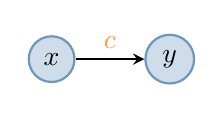
\begin{tikzpicture}[auto]

%
% Styles
%
\tikzstyle{vertex} = [circle,draw=oproverblue!60,fill=oproverblue!20,thick]
\tikzstyle{edge}   = [->,>=stealth,thick]
\tikzstyle{weight} = [color=oproveryellow]

\node[vertex] (x) at (2,0)   {$x$};
\node[vertex] (y) at (3.5,0) {$y$};

\draw[edge] (x) -- node[weight] {$c$} (y);

\end{tikzpicture}

  \end{center}

  \pause
  \vfill
  So, a set $\babst{\mu}$ can be encoded as a graph. Concrete example:

  \begin{columns}

    \begin{column}{.3\textwidth}
      \ra{1.3}
      $$
      \begin{array}{rcr}
	x - y & \leq & 8   \\
	y - z & \leq & -1  \\
	z - x & \leq & -6  \\
	z - w & \leq & 2   \\
	w - x & \leq & -10 \\
	w - t & \leq & 0   \\
	t - x & \leq & 3     
      \end{array}
      $$
    \end{column}

    \begin{column}{.6\textwidth}
      \begin{center}
	\begin{frame}
  \frametitle{An Example}

  \scriptsize

  Consider the following problem

  \begin{overlayarea}{\textwidth}{1cm}
    \only<1|handout:0>{$$ x_1 - x_2 \leq 8\ \swedge\ x_2 - x_3 \leq -1\ \swedge\ x_3 - x_4 \leq 2\ \swedge\ x_4 - x_1 \leq -10 $$} 
    \only<2->{$$ x_5 \leq 8\ \swedge\ x_6 \leq -1\ \swedge\ x_7 \leq 2\ \swedge\ x_8 \leq -10 $$} 
  \end{overlayarea}

  \onslide<2->{
  \begin{columns}

  \begin{column}{.4\textwidth}
  \begin{center}
  Tableau
  \end{center}
  $$
  \only<2-4|handout:0>{
  \begin{array}{rcl}
    x_5 & = & x_1 - x_2  \\ 
    x_6 & = & x_2 - x_3  \\ 
    x_7 & = & x_3 - x_4  \\ 
    x_8 & = & x_4 - x_1  \\ 
  \end{array}}
  \only<5-7|handout:0>{
  \begin{array}{rcl}
    x_5 & = & x_1 - x_2  \\ 
    x_3 & = & x_2 - x_6  \\ 
    x_7 & = & x_2 - x_6 - x_4  \\ 
    x_8 & = & x_4 - x_1  \\ 
  \end{array}}
  \only<8|handout:0>{
  \begin{array}{rcl}
    x_5 & = & x_4 - x_8 - x_2  \\ 
    x_3 & = & x_2 - x_6  \\ 
    x_7 & = & x_2 - x_6 - x_4  \\ 
    x_1 & = & x_4 - x_8  \\ 
  \end{array}}
  \only<9,10>{
  \begin{array}{rcl}
    x_2 & = & x_4 - x_8 - x_5  \\ 
    x_3 & = & x_4 - x_8 - x_5 - x_6  \\ 
    \coloneat{x_7}{10} & \coloneat{=}{10} & \coloneat{- x_5 -x_8 - x_6}{10} \\ 
    x_1 & = & x_4 - x_8  \\ 
  \end{array}}
  $$
  \end{column}

  \begin{column}{.3\textwidth}
  \begin{center}
  $lb$~~~~~~~Bounds~~~~~~~$ub$
  \end{center}
  $$
  \begin{array}{rcccl}
    - \infty & \leq & x_5 & \leq & \only<2|handout:0>{\infty}\only<3->{8} \\
    - \infty & \leq & x_6 & \leq & \only<2,3|handout:0>{\infty}\only<4->{-1} \\
    - \infty & \leq & x_7 & \leq & \only<2-5|handout:0>{\infty}\only<6->{2} \\
    - \infty & \leq & x_8 & \leq & \only<2-6|handout:0>{\infty}\only<7->{-10} \\
  \end{array}
  $$
  \end{column}

  \begin{column}{.3\textwidth}
  \begin{center}
  $\mu$
  \end{center}
  $$
  \begin{array}{rcl}
  x_1 & \mapsto & \only<2-7|handout:0>{0}\only<8->{10} \\
  x_2 & \mapsto & \only<2-8|handout:0>{0}\only<9->{2} \\
  x_3 & \mapsto & \only<2-4|handout:0>{0}\only<5->{1} \\
  x_4 & \mapsto & 0 \\ 
  x_5 & \mapsto & \only<2-7|handout:0>{0}\only<8|handout:0>{10}\only<9->{8} \\
  x_6 & \mapsto & \only<2-4|handout:0>{0}\only<5->{-1} \\
  x_7 & \mapsto & \only<2-4|handout:0>{0}\only<5-8|handout:0>{1}\only<9->{3} \\
  x_8 & \mapsto & \only<2-7|handout:0>{0}\only<8->{-10} 
  \end{array}
  $$
  \end{column}

  \end{columns}
  }
  \vfill
  \begin{overlayarea}{\textwidth}{1cm}
    \only<3|handout:0>{Receiving $x_5 \leq 8$: OK}
    \only<4|handout:0>{Receiving $x_6 \leq -1$: $\mu(x_6)$ out of bounds}
    \only<5|handout:0>{$Pivot(x_6,x_3)$, $Update(x_6,-1)$. Values of $x_3$ and $x_7$ change as well}
    \only<6|handout:0>{Receiving $x_7 \leq 2$: OK}
    \only<7|handout:0>{Receiving $x_8 \leq -10$: $\mu(x_8)$ out of bounds}
    \only<8|handout:0>{$Pivot(x_8,x_1)$, $Update(x_8,-10)$. Values of $x_5$ and $x_1$ change as well. $\mu(x_5)$ out of bounds}
    \only<9|handout:0>{$Pivot(x_5,x_2)$, $Update(x_5,8)$. Values of $x_2$ and $x_7$ change as well. $\mu(x_7)$ out of bounds}
    \only<10>{Cannot find suitable variable for pivoting ($ChoosePivot(x_7)$ == $undef$). Return $unsat$}
  \end{overlayarea}

\end{frame}

      \end{center}
    \end{column}

  \end{columns}
  \vfill
  $G( V, E )$: $V = \{ x, y, z, w, t \}$, $E = \{ (x,y;8), (y,z;-1), (z,x;-6), (z,w;2), (w,x;-10), \ldots \}$ 

\end{frame}

\begin{frame}
  \frametitle{Translation into a Graph}

  \scriptsize

    \begin{theorem}[Translation]
      \label{the:idl}
      $\babst{\mu}$ is \Idl-unsatisfiable 
      \begin{center}
      iff
      \end{center}
      there is a {\bf negative cycle} in the corresponging graph $G(V,E)$
    \end{theorem}

  \pause
  \vfill
  E.g.:

  \begin{columns}

    \begin{column}{.3\textwidth}
      \ra{1.3}
      $$
      \begin{array}{rcr}
	\coloneat{x - y}{3-} & \coloneat{\leq}{3-} & \coloneat{8}{3-}   \\
	\coloneat{y - z}{3-} & \coloneat{\leq}{3-} & \coloneat{-1}{3-}  \\
	\colfouat{z - x}{3-} & \colfouat{\leq}{3-} & \colfouat{-6}{3-}  \\
	\coloneat{z - w}{3-} & \coloneat{\leq}{3-} & \coloneat{2}{3-}   \\
	\coloneat{w - x}{3-} & \coloneat{\leq}{3-} & \coloneat{-10}{3-} \\
	\colfouat{w - t}{3-} & \colfouat{\leq}{3-} & \colfouat{0}{3-}   \\
	\colfouat{t - x}{3-} & \colfouat{\leq}{3-} & \colfouat{3}{3-}     
      \end{array}
      $$
    \end{column}

    \begin{column}{.6\textwidth}
      \begin{center}
	\begin{overlayarea}{.5\textwidth}{3cm}
	  \only<2|handout:0>{\begin{frame}
  \frametitle{An Example}

  \scriptsize

  Consider the following problem

  \begin{overlayarea}{\textwidth}{1cm}
    \only<1|handout:0>{$$ x_1 - x_2 \leq 8\ \swedge\ x_2 - x_3 \leq -1\ \swedge\ x_3 - x_4 \leq 2\ \swedge\ x_4 - x_1 \leq -10 $$} 
    \only<2->{$$ x_5 \leq 8\ \swedge\ x_6 \leq -1\ \swedge\ x_7 \leq 2\ \swedge\ x_8 \leq -10 $$} 
  \end{overlayarea}

  \onslide<2->{
  \begin{columns}

  \begin{column}{.4\textwidth}
  \begin{center}
  Tableau
  \end{center}
  $$
  \only<2-4|handout:0>{
  \begin{array}{rcl}
    x_5 & = & x_1 - x_2  \\ 
    x_6 & = & x_2 - x_3  \\ 
    x_7 & = & x_3 - x_4  \\ 
    x_8 & = & x_4 - x_1  \\ 
  \end{array}}
  \only<5-7|handout:0>{
  \begin{array}{rcl}
    x_5 & = & x_1 - x_2  \\ 
    x_3 & = & x_2 - x_6  \\ 
    x_7 & = & x_2 - x_6 - x_4  \\ 
    x_8 & = & x_4 - x_1  \\ 
  \end{array}}
  \only<8|handout:0>{
  \begin{array}{rcl}
    x_5 & = & x_4 - x_8 - x_2  \\ 
    x_3 & = & x_2 - x_6  \\ 
    x_7 & = & x_2 - x_6 - x_4  \\ 
    x_1 & = & x_4 - x_8  \\ 
  \end{array}}
  \only<9,10>{
  \begin{array}{rcl}
    x_2 & = & x_4 - x_8 - x_5  \\ 
    x_3 & = & x_4 - x_8 - x_5 - x_6  \\ 
    \coloneat{x_7}{10} & \coloneat{=}{10} & \coloneat{- x_5 -x_8 - x_6}{10} \\ 
    x_1 & = & x_4 - x_8  \\ 
  \end{array}}
  $$
  \end{column}

  \begin{column}{.3\textwidth}
  \begin{center}
  $lb$~~~~~~~Bounds~~~~~~~$ub$
  \end{center}
  $$
  \begin{array}{rcccl}
    - \infty & \leq & x_5 & \leq & \only<2|handout:0>{\infty}\only<3->{8} \\
    - \infty & \leq & x_6 & \leq & \only<2,3|handout:0>{\infty}\only<4->{-1} \\
    - \infty & \leq & x_7 & \leq & \only<2-5|handout:0>{\infty}\only<6->{2} \\
    - \infty & \leq & x_8 & \leq & \only<2-6|handout:0>{\infty}\only<7->{-10} \\
  \end{array}
  $$
  \end{column}

  \begin{column}{.3\textwidth}
  \begin{center}
  $\mu$
  \end{center}
  $$
  \begin{array}{rcl}
  x_1 & \mapsto & \only<2-7|handout:0>{0}\only<8->{10} \\
  x_2 & \mapsto & \only<2-8|handout:0>{0}\only<9->{2} \\
  x_3 & \mapsto & \only<2-4|handout:0>{0}\only<5->{1} \\
  x_4 & \mapsto & 0 \\ 
  x_5 & \mapsto & \only<2-7|handout:0>{0}\only<8|handout:0>{10}\only<9->{8} \\
  x_6 & \mapsto & \only<2-4|handout:0>{0}\only<5->{-1} \\
  x_7 & \mapsto & \only<2-4|handout:0>{0}\only<5-8|handout:0>{1}\only<9->{3} \\
  x_8 & \mapsto & \only<2-7|handout:0>{0}\only<8->{-10} 
  \end{array}
  $$
  \end{column}

  \end{columns}
  }
  \vfill
  \begin{overlayarea}{\textwidth}{1cm}
    \only<3|handout:0>{Receiving $x_5 \leq 8$: OK}
    \only<4|handout:0>{Receiving $x_6 \leq -1$: $\mu(x_6)$ out of bounds}
    \only<5|handout:0>{$Pivot(x_6,x_3)$, $Update(x_6,-1)$. Values of $x_3$ and $x_7$ change as well}
    \only<6|handout:0>{Receiving $x_7 \leq 2$: OK}
    \only<7|handout:0>{Receiving $x_8 \leq -10$: $\mu(x_8)$ out of bounds}
    \only<8|handout:0>{$Pivot(x_8,x_1)$, $Update(x_8,-10)$. Values of $x_5$ and $x_1$ change as well. $\mu(x_5)$ out of bounds}
    \only<9|handout:0>{$Pivot(x_5,x_2)$, $Update(x_5,8)$. Values of $x_2$ and $x_7$ change as well. $\mu(x_7)$ out of bounds}
    \only<10>{Cannot find suitable variable for pivoting ($ChoosePivot(x_7)$ == $undef$). Return $unsat$}
  \end{overlayarea}

\end{frame}
}
	  \only<3->{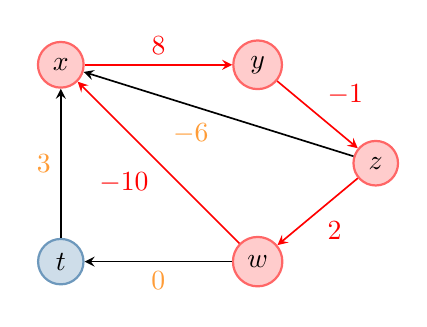
\begin{tikzpicture}[auto]

%
% Styles
%
\tikzstyle{vertex}   = [circle,draw=oproverblue!60,fill=oproverblue!20,thick]
\tikzstyle{edge}     = [->,>=stealth,semithick]
\tikzstyle{weight}   = [color=oproveryellow]
\tikzstyle{hlvertex} = [circle,draw=red!60,fill=red!20,thick]
\tikzstyle{hledge}   = [->,>=stealth,semithick,draw=red]
\tikzstyle{hlweight} = [color=red]

\node[hlvertex] (x) at (  1, 0)    {$x$};
\node[hlvertex] (y) at (3.5, 0)    {$y$};
\node[hlvertex] (z) at (  5,-1.25) {$z$};
\node[hlvertex] (w) at (3.5,-2.5)  {$w$};
\node[vertex] (t) at (  1,-2.5)  {$t$};

\draw[hledge] (x) -- node[hlweight] {$8$}   (y);
\draw[hledge] (y) -- node[hlweight] {$-1$}  (z);
\draw[edge]   (z) -- node[weight] {$-6$}  (x);
\draw[hledge] (z) -- node[hlweight] {$2$}   (w);
\draw[hledge] (w) -- node[hlweight] {$-10$} (x);
\draw[edge]   (w) -- node[weight] {$0$}   (t);
\draw[edge]   (t) -- node[weight] {$3$}   (x);

\end{tikzpicture}
}
	\end{overlayarea}
      \end{center}
    \end{column}

  \end{columns}

\end{frame}

\begin{frame}
  \frametitle{Translation into a Graph}

  We use the following lemma to aid the proof

  \begin{lemma}[Farka's Lemma for \Idl]
    $\babst{\mu}$ is unsatisfiable iff there exists a subset 
    $\babst{\nu} = \{\ \coltwo{x_1} - x_2 \leq c_1,\ x_2 - x_3 \leq c_2,\ \ldots,\ x_n - \coltwo{x_1} \leq c_n\ \}$ of $\babst{\mu}$
    such that $c_1 + \ldots + c_n < 0$
  \end{lemma}
  \pause
  \vfill
  The proof of Theorem is now trivial
  \begin{proof}
  $\babst{\mu}$ is unsatisfiable iff \colfou{by Farka's Lemma for \Idl} \\
  there exists $\babst{\nu} \subseteq \babst{\mu}$ with $c_1 + \ldots + c_n < 0$ iff \colfou{by our translation} \\
  there exists a negative cycle in $G(V,E)$
  \end{proof}

\end{frame}

\begin{frame}
  \frametitle{Handling Functions}

  \scriptsize

  Let's consider also function symbols. We want to extend Union-Find
  to handle functions as well. For instance 
  $$x=y\ \wedge\ f(x)=z\ \wedge\ f(y)=w$$
  should result into
  $$
  \{\ x,\ y\ \}\quad\quad\quad\quad\{\ f(x),\ f(y),\ z,\ w\ \}
  $$
  \vfill\pause
  We don't see the details, but just a generic algorithm. Let 
  $\varphi^+$ be a conjunction of positive equalities between \Uf-terms
  \begin{tabbing}
  asd \= as \= as \= as \= as \kill
  1 \> {\bf procedure} Congruence-Closure( $\varphi^+$ ) \\
  2 \> $pending = \varphi^+$ \\
  3 \> while ( $pending$ not empty ) \\  
  4 \> \> $(s = t) = pending$.pop( ) \\
  5 \> \> $s =$ Find( $s$ ) \\
  6 \> \> $t =$ Find( $t$ ) \\
  7 \> \> Union( $s$, $t$ ) \\
  8 \> \> for each pair $p$, $q$ such that\\
    \> \> \> \> 1. Find( $p$ ) $\not\equiv$ Find( $q$ ) \\
    \> \> \> \> 2. $p \equiv f( s_1, \ldots, s_n )$,\ \ $q \equiv f( t_1, \ldots, t_n )$ \\
    \> \> \> \> 3. Find($s_1$)=Find($t_1$),\ldots,Find($s_n$)=Find($t_n$) \\
  9 \> \> \> $pending$.push( $p=q$ ) \\
 \end{tabbing}
 \vfill\pause
 After Congruence-Closure we have that
 \begin{center}
   $s$, $t$ are in the same partition iff $\varphi^+ \Rightarrow s=t$
 \end{center}

\end{frame}

\begin{frame}
  \frametitle{Example}

  \scriptsize

 $\varphi^+ \equiv f(a,b)=a\ \wedge\ f(f(a,b),b)=c$
 \vfill
 $pending = \{\quad f(a,b)=a,\quad f(f(a,b),b)=c\quad \}$ 
 $$
 \{\ a\ \}\quad\quad\{\ b\ \}\quad\quad\{\ c\ \}\quad\quad\{\ f(a,b)\ \}\quad\quad\{\ f(f(a,b),b)\ \}
 $$
 \vfill
 $pending = \{\quad f(f(a,b),b)=c\quad f(f(a,b),b)=f(a,b)\quad \}$ 
 $$
 \{\ a, f(a,b)\ \}\quad\quad\{\ b\ \}\quad\quad\{\ c\ \}\quad\quad\{\ f(f(a,b),b)\ \}
 $$
 \vfill
 $pending = \{\quad f(f(a,b),b)=f(a,b)\quad \}$ 
 $$
 \{\ a, f(a,b)\ \}\quad\quad\{\ b\ \}\quad\quad\{\ f(f(a,b),b), c\ \}
 $$
 \vfill
 $pending = \{ \}$ 
 $$
 \{\ a, f(a,b), f(f(a,b),b), c\ \}\quad\quad\{\ b\ \}
 $$

\end{frame}

\begin{frame}
  \frametitle{Solving}

  Finally we are ready to check satisfiability of $\varphi$. As before
  $\varphi \equiv \varphi^+ \wedge \varphi^-$. Negated equalities can
  be checked after building equivalence classes
  \vfill
  \begin{tabbing}
  asd \= as \= as \= as \= as \kill
  1 \> {\bf procedure} Check( $\varphi^+$, $\varphi^-$ ) \\
  2 \> Congruence-Closure( $\varphi^+$ ) \\
  3 \> for each $s \not= t$ in $\varphi^-$ \\
  4 \> \> $s' =$ Find( $s$ ) \\
  5 \> \> $t' =$ Find( $t$ ) \\
  6 \> \> if ( $s' \equiv t'$ ) \\
  7 \> \> \> return $unsat$ \\
  8 \> return $sat$ 
 \end{tabbing}
 \vfill\pause
 This is correct, because
 \begin{itemize}
   \item at line 3, $s$, $t$ are in the same partition iff $\varphi^+ \Rightarrow s=t$
   \item at line 7, $s$, $t$ are in the same partition, but $s\not=t$
 \end{itemize}

\end{frame}


\begin{frame}
  \frametitle{Outline}
  \tableofcontents
\end{frame}

\section{Improvement for \tsolver}
\begin{frame}
  \frametitle{\tsolver Compliance}

  So far we have seen that BF can be used
  to compute a model of a given {\bf consistent}
  set of \Idl constraints
  \vfill
  Recall that to have an efficient \tsolver
  the following features should be supported
  \vfill
  \begin{itemize}
    \item Minimal Conflicts
  \vfill
    \item Incrementality
  \vfill
    \item Backtrackability
  \vfill
    \item Theory Propagation
  \end{itemize}
  \vfill
  Let's see how to improve the current algorithm to
  support them

\end{frame}

\subsection{Minimal Conflicts}

\begin{frame}
  \frametitle{Minimal Conflicts}

  So far we assumed that $G(V,E)$ did not contain
  negative cycles. However it is not difficult to
  tweak the BF to recognize them
  \vfill
  \pause
  Recall the {\bf spanning tree}: the tree that holds
  shortest paths 
  \vfill
  \begin{center}
    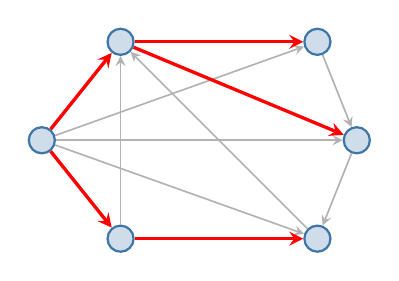
\begin{tikzpicture}[auto]

%
% Styles
%
\tikzstyle{nonvertex} = [circle,draw=white,fill=white,thick,color=white]
\tikzstyle{vertex} = [circle,draw=oproverblue!80,fill=oproverblue!20,thick]
\tikzstyle{edge}   = [->,>=stealth,semithick,draw=grey,color=grey]
\tikzstyle{edge0}  = [->,>=stealth,semithick,draw=grey]
\tikzstyle{edge1}  = [->,>=stealth,very thick,draw=red,color=red]
\tikzstyle{weight} = [color=oproveryellow]
\tikzstyle{hlvertex} = [circle,draw=mydarkgreen!60,fill=mydarkgreen!20,thick]

\node[vertex] (x) at (  1, 0)     {};
\node[vertex] (y) at (3.5, 0)     {};
\node[vertex] (z) at ( 4,-1.25)   {};
\node[vertex] (w) at (3.5,-2.5)   {};
\node[vertex] (t) at (  1,-2.5)   {};
\node[vertex] (I) at (  0, -1.25) {};

\draw[edge1] (I) -- (x);
\draw[edge]  (I) -- (y);
\draw[edge]  (I) -- (z);
\draw[edge] (I) -- (w);
\draw[edge1] (I) -- (t);

\draw[edge1] (x) -- (y);
\draw[edge] (y) -- (z);
\draw[edge1] (x) -- (z);
\draw[edge]  (z) -- (w);
\draw[edge] (w) -- (x);
\draw[edge1]  (t) -- (w);
\draw[edge]  (t) -- (x);

\end{tikzpicture}

  \end{center}
  \vfill
  \pause
  It is easy to keep the spanning tree:
  \begin{itemize}
    \item each node $t$ keeps two fields {\bf fatherVertex}
	  and {\bf fatherEdge} that stores its father 
          in the spanning tree
    \item when a {\bf relax} is done on $t$ (line 8 of BF)
	  through an edge $e = (s, t; c)$, $t.fatherVertex$ is
	  set to $s$ and $t.fatherEdge$ is set to $e$
  \end{itemize}

\end{frame}

\begin{frame}
  \frametitle{Minimal Conflicts}

  \scriptsize

  When a negative cycle exists, the spanning tree tends
  to become {\bf cyclic} (trees are acyclic instead). It is
  easy to recognize this situation and report the negative cycle

  \vfill
  \pause

  \begin{columns}

  \begin{column}{.45\textwidth}
    $TBV =$ [ ] \\
    Current vetex: $z$ \\
    Current edge: $(z,w;2)$ 
  \end{column}

  \begin{column}{.45\textwidth}
    \begin{center}
    \begin{overlayarea}{\textwidth}{3cm}
      \input{neg_cycle_1}
    \end{overlayarea}
    \end{center}
  \end{column}

  \end{columns}

  \vfill
  \pause

  \begin{tabbing}
  as \= a \= a \= a \= as \= asdfasdfasdfasdfasdfasdfasdfasdf \= \kill
  checkNegativeCycle( $s$, $t$ ) \\
  \> $\babst{\nu} = \{ \ \}$ \\ \\
  \> while ( $s \not= t$ \&\& $s \not= I$ ) \\
  \> \> $s = s.fatherVertex$ \\
  \> \> $\babst{\nu} = \babst{\nu} \cup \{ s.fatherEdge \}$ \\ \\
  \> if ( $s$ == $t$ ) return conflict \>\>\>\>\> // Neg. Cycle detected \\
  \> return OK        \>\>\>\>\> // $I$ reached
  \end{tabbing}

\end{frame}

\begin{frame}
  \frametitle{Minimal Conflicts}

  Bellman-Ford with negative cycle detection

  \begin{tabbing}
  as \= a \= a \= a \= as \= asdfasdfasdfasdfasdfasdfasdfasdf \= \kill
  1  \> $\pi(x) = \infty$ for all $x \in V, x \not= I$ \\
  2  \> $\pi(I) = 0$ \\
  3  \> $TBV.pushBack( I )$ \\
  4  \> while ( $TBV.size(\ ) > 0$ ) \\
  5  \> \> $s = TBV.popFront(\ )$ \\
  6  \> \> foreach $(s,t;w) \in E$         \> \> \> \> // for each outgoing edge \\
  7  \> \> \> if ( $\pi(t) - \pi(s) > w$ )    \> \> \> // is too far ? \\
  8  \> \> \> \> \colone{if ( checkNegativeCycle( $s$, $t$ ) == conflict )} \\
  9  \> \> \> \> \> \colone{return $\babst{\nu}$} \\
  10 \> \> \> \> \colone{$s.fatherVertex = t$} \\
  11 \> \> \> \> \colone{$s.fatherEdge = (s,t;w)$} \\
  12  \> \> \> \> $\pi(t) = \pi(s) + w$           \> \> // relax (decrease $\pi(t)$) \\
  13  \> \> \> \> if ( $TBV.has( t ) == false$ ) \\ 
  14 \> \> \> \> \> $TBV.pushBack( t )$             \> // enqueue $t$ if not there \\
  \end{tabbing}

\end{frame}

\subsection{Incrementality}

\begin{frame}
  \frametitle{Incrementality}

  \scriptsize
  
  Incrementality comes almost for free !
  \vfill
  \begin{itemize}

    \item we always keep the $\pi$ function ``alive'', and only
          update it slightly
  \vfill

    \item $G(V,E)$ keeps track of {\bf active} and {\bf inactive}
          edges: active edges are those on $\babst{\mu}$
  \vfill

    \item when a new \tatom $x - y \leq c$ is added to $\babst{\mu}$, the
	  corresponding edge $(x,y;c)$ becomes active in the graph
  \vfill

    \item we add $x$ to $TBV$, and run BF from line 4

  \end{itemize}
  \vfill
  \begin{columns}

  \begin{column}{.3\textwidth}
  \begin{center}
    $x-y \leq 8 \not\in \babst{\mu}$ \\
    \medskip
    \scalebox{.7}{\input{incremental}}
  \end{center} 
  \end{column}

  \pause

  \begin{column}{.3\textwidth}
  \begin{center}
    $x-y \leq 8$ pushed to $\babst{\mu}$ \\
    \medskip
    \scalebox{.7}{\input{incremental_1}}
  \end{center} 
  \end{column}

  \pause

  \begin{column}{.3\textwidth}
  \begin{center}
    After BF \\
    \medskip
    \scalebox{.7}{\input{incremental_2}}
  \end{center} 
  \end{column}

  \end{columns}

\end{frame}

\subsection{Backtrackability}

\begin{frame}
  \frametitle{Backtrackability}

  Backtracking can be done efficiently
  \vfill
  First of all, recall that $\mu(x) = -\pi(x)$. Second obeserve that
  \vfill
  \begin{exampleblock}{Observation 1}
    Let $\mu$ be a model for a set $\babst{\mu}$ of constraints.
    Then $\mu$ is also a model for {\bf any subset} of $\babst{\mu}$
  \end{exampleblock}
  \vfill
  Observation 1 implies that when backtracking we just have to turn some
  edges into inactive, and keep the last $\pi$ intact
  \vfill
  This is done as follows: BF will always work on a temporary $\pi$, called $\pi'$. If satisfiable,
  $\pi$ is replaced by $\pi'$, otherwise we keep $\pi$  

\end{frame}

\subsection{Theory Propagation}

\begin{frame}
  \frametitle{Theory Propagation}

  Theory Propagation is the process of activating some edges in the
  graph that are implied by the current $\babst{\mu}$
  \vfill
  \begin{exampleblock}{Observation 2}
    A set of constraints \\
    $\{\ \colone{x_1} - x_2 \leq c_1,\ x_2 - x_3 \leq c_2,\ \ldots,\ x_{n-1} - \coltwo{x_n} \leq c_{n-1}\ \}$ \\
    implies 
    $\quad\quad\colone{x_1} - \coltwo{x_n} \leq c_n\quad\quad$ 
    iff 
    $\quad\quad c_1 + c_2 + \ldots c_{n-1} \leq c_n$
  \end{exampleblock}
  \vfill
  \pause
  Example:

  \begin{center}
    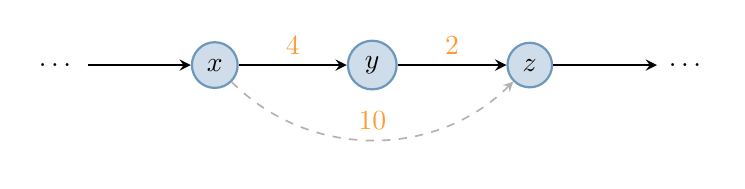
\begin{tikzpicture}[auto]

%
% Styles
%
\tikzstyle{vertex} = [circle,draw=oproverblue!60,fill=oproverblue!20,thick]
\tikzstyle{edge}   = [->,>=stealth,thick]
\tikzstyle{edge2}  = [->,>=stealth,semithick,draw=grey,color=grey,dashed]
\tikzstyle{weight} = [color=oproveryellow]

\node[vertex] (x) at (0,0)   {$x$};
\node[vertex] (y) at (2,0)   {$y$};
\node[vertex] (z) at (4,0)   {$z$};
\node[circle] (h) at (-2,0)   {\ldots};
\node[circle] (k) at (6,0)    {\ldots};

\draw[edge]  (x) -- node[weight] {$4$} (y);
\draw[edge]  (y) -- node[weight] {$2$} (z);
\draw[edge]  (h) -- (x);
\draw[edge]  (z) -- (k);
\draw[edge2] (x) to [out=-45,in=225] node[weight] {$10$} (z);

\end{tikzpicture}
 
  \end{center}

  $x - z \leq 10$, currently inactive, can be theory-propagated

\end{frame}


\section{Final Remarks}
\begin{frame}
  \frametitle{Exercizes}

  \begin{enumerate}

    \item Show that the \tconflicts generated by the Simplex are minimal

    \vfill
    \item Suppose that $(0,1) \leq x \leq (1,-1)$. Compute the biggest possible value for $\delta$

    \vfill
    \item Find the candidate for pivoting in this row (for simplicity we use normal numbers)
	  $$
	  x_1 = 3 x_2 - 9 x_3 - 7 x_4
	  $$
	  given these bounds $-\infty \leq x_1 \leq 1$, $0 \leq x_2 \leq \infty$, $- \infty \leq x_3 \leq -1$, $1 \leq x_4 \leq 2$
	  and this assignment $\mu = \{ x_1 \mapsto \colone{2}, x_2 \mapsto 0, x_3 \mapsto -1, x_4 \mapsto 1 \}$
    \vfill

    \item Using the row of previous exercize, change the bounds
          so that the only candidate for pivoting becomes $x_2$

    \item Now change the bounds so that no pivoting is possible.
          Compute the conflict

  \end{enumerate}

\end{frame}


\end{document}
